\section{Background Monte Carlo} \label{sec:data:bkg_mc}

Modeling the expected contributions of backgrounds to the analysis is also done
with the use of Monte Carlo simulated samples.  These were used for the
development of the modeling of the non-resonant QCD multi-jet backgrounds, and
for the estimation of the major resonant backgrounds from $V$+jet, $t\bar{t}$
shown in figure \Cref{simulated_background_shapes} and single-top.  For the
multi-jet background the final esimation is data drive, but the MC was used to
develop the estimation model.

\begin{figure}[!htbp]
  \centering
  \subcaptionbox{Simulation of the contribution of non-resonant multijet QCD background in the signal region.}{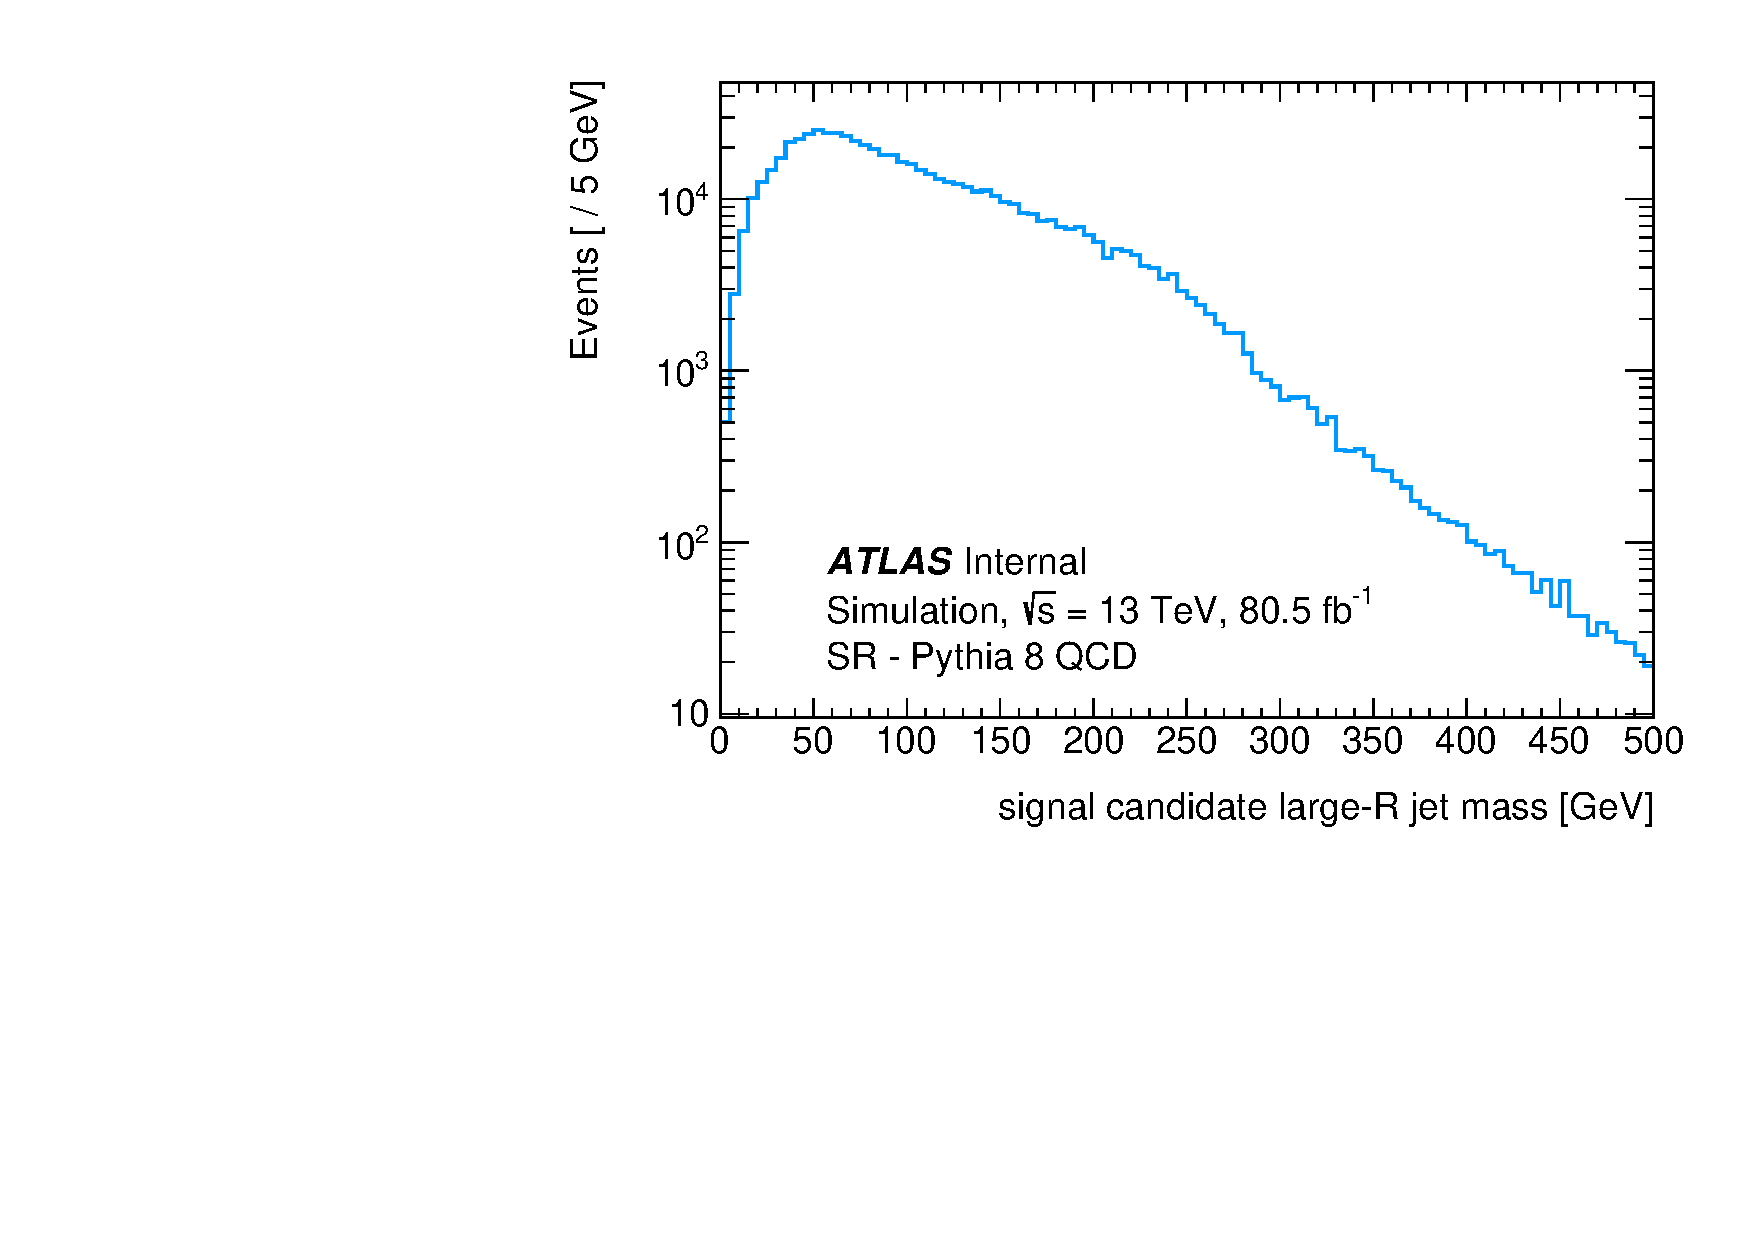
\includegraphics[width=0.49\linewidth]{figures/data/QCD_logy}} \hfill
  \subcaptionbox{Simulation of resonant $V$+jets and $t\bar{t}$ backgrounds in the signal region.  The Higgs simulation is included for comparison.}{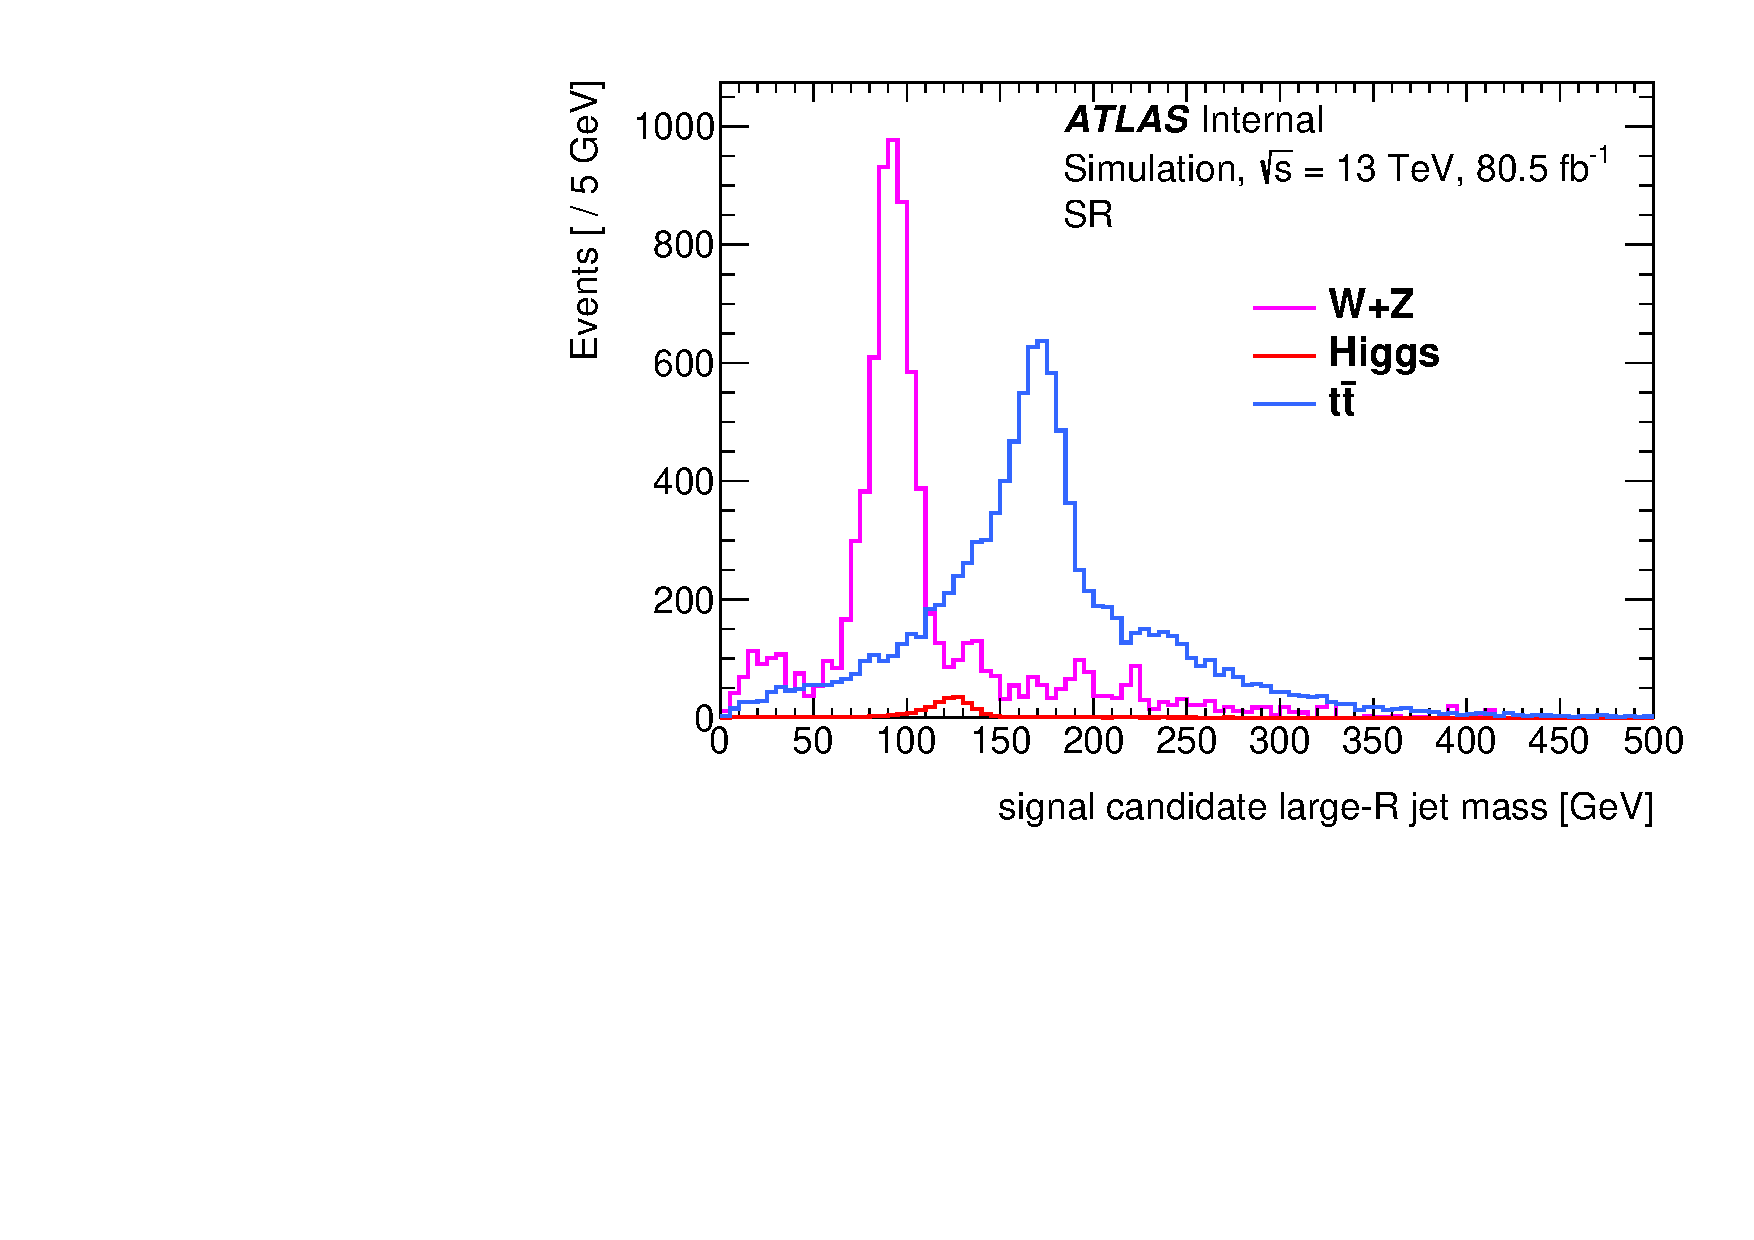
\includegraphics[width=0.49\linewidth]{figures/data/resonant_bkg}}
  \caption{Simulations of the non-resonant and resonant background contributions to the signal region for an integrated luminosity of $80.5\text{fb}^{-1}$}
  \label{simulated_background_shapes}
\end{figure}

The QCD dijet events were simulated using the \textsc{Pythia} 8.186
\cite{Sjostrand:2007gs} generator with the A14 tune and the NNPDF23 LO
PDF~\cite{Carrazza:2013axa} using EvtGen~\cite{LANGE2001152} to decay
the resulting $b$-hadrons.  To maintian a constant statistical precision over
a large energy range the weighted events were generated using a flat \pT
spectrum.

Hadronically decaying $W$ and $Z$ events were produced with a mamximum of 4
four additional partons at Leading Order (LO).  This was accomplished with the
\textsc{Sherpa} 2.1.1~\cite{Gleisberg:2008ta} generator and the CT10
\cite{Lai:2010vv} parton distribution function.  For Leptonically decaying $W$
and $Z$ events we were able to produce samples with a maximum of two additional
partons at LO and a maximum of four at Next to Leading Order (NLO).  This
allowed us to correct the LO hadronic $W$ and $Z$ cross-sections to the NLO
leptonic $W$ and $Z$ cross-sections by applying multiplicative "$k$-factors".
These corrections were 1.28 for the $W$+jets and 1.37 for the $Z$+jets
\cite{Aaboud:2018zba}. An alternate set of Hadronically decaying $W$ and $Z$
events was produced for cross checks using the
\text{Herwig}++2.7.1~\cite{Bahr:2008pv} generator with the
UEEE4~\cite{Buckley:2018wdv} tune and the CTEQ6L1~\cite{Pumplin:2002vw}. Unlike
the \textsc{Sherpa} samples these \textsc{Herwig} samples only contained one
additional parton in the matrix element calculation.

Our $t\bar{t}$ samples were generated at tree-level using
\textsc{Powheg-Box}~\cite{Campbell2012} 2 and the NNPDF30
NLO~\cite{Ball:2014uwa} parton distribution function. After generation the
events were showered using \textsc{Pythia} 8.230~\cite{Sjostrand:2014zea} using
the A14 tune and the NNPDF23 LO~\cite{Carrazza:2013axa} parton
distribution function with all $b$-hadron decays performed by
EvtGen~\cite{LANGE2001152}.  The samples were then broken up according to the
decay mode of the two top quarks into three categories; all-hadronic,
semi-leptonic, all-leptonic. An additional sample of $t\bar{t}$ event were
generated using \textsc{Sherpa} 2.2.1~\cite{Gleisberg:2008ta} using the NNPDF30
NNLO~\cite{Ball:2014uwa} parton distribution.  This second sample was used as a
cross check to the main samples generated with \textsc{Powheg-Box} 2 +
\textsc{Pythia} 8.

Single-top samples, containing a single top/anti-top quark and a
$W^{-}$/$W^{+}$, were generated at tree-level with \textsc{Powheg-Box}
2~\cite{Campbell2012} with the NNPDF30~\cite{Lai:2010vv} parton distribution
function. This process was showered using \textsc{Pythia}
8.230~\cite{Sjostrand:2014zea} configured with the A14 tune, the
NNPDF23~\cite{Carrazza:2013axa} parton distribution with all resulting
$b$-hadrons decayed via EvtGen~\cite{LANGE2001152}.
